\documentclass[11pt,a4paper]{report}
\usepackage{graphics,graphicx}
\usepackage{hyperref}
\usepackage{fullpage}
\usepackage{pdflscape}
\usepackage{tikz}
\usepackage{setspace}
\usepackage{enumitem}
\usepackage{index}
\makeindex
\onehalfspacing

\usepackage{graphicx}
\begin{document}

\title{Interactive Graduate Student Information Database: Midterm Report} 
\author{Kartik Thakore (250313003)\\kthakore@uwo.ca}
\maketitle

\tableofcontents
\clearpage
\newpage
\chapter{Software Specifications}
\section{Introduction}
\index{purpose}
\subsection{Purpose}
The purpose of this report is to document preliminary elicited requirements for the Interactive Graduate Student Information System (SIMS). Additionally, in accordance with the Agile project management
methodology, a walk through of the first iteration is documented. Our first iteration includes two system
critical features which will be used for iterative system development of the system. Database schemas and
operational logic for user authentication and calculations for graduate student funding were accomplished.
A database schematic was designed after performing extensive analysis based on our specifications, data flow
requirements and approved system critical assumptions. Data normalization was performed and a Representational State Transfer (REST) framework was implemented to combine components. Furthermore, unit and
integration testing were performed with the preliminary implementation in place. For preparation of future
iterations, a sign-off from end users and client is required. However, we have started the rapid prototyping
of the e-signature component for the advisory meeting tracking feature.
\subsection{Scope}
\index{scope}
\index{BioMedical Physics}
The scope of the following requirements is to provide a pilot software back end for the BioMedical Physics
Graduate program at UWO. First the system will replace the current method of tracking student information
pictured in Figure \ref{fig:Curr_Sys}.
\begin{itemize}
\item The current system provides the following features which directly fall into scope for this product:
\begin{itemize}
\item Storage of Intrinsic Student Value
\item Graphical User Interface for Entering Student Data
\item Saving portable reports for external users
\end{itemize}
\item The new system will additionally need to address the following concerns:
\begin{itemize} 
\item Store data securely and with more redundancy
\item Simply the User Interface for using the system
\item Remove the load of managing data solely on one user
\item Allow faculty members to view data in a meaningful way
\item Allow students to update their information
\item Allow advisory committee members to store and retrieve signatures and comments on the system
\end{itemize} 
\end{itemize}
Currently the scope is limited to tackling these core issues. However since the project cycle is iterative,
the scope can be expanded in a controlled manner, should the situation demand it.
\subsection{Definitions, acronyms, and abbreviations}
\begin{itemize}
\item SIMS: Student Information System
\item UWO: University of Western Ontario
\item REST: Software Architecture for Web Applications
\item VPN: Virtual Private Network
\item SSL: Security Protocol for Web Applications
\end{itemize}
\subsection{ References }
\subsection{ Overview }
The SIMS core is a secure application that aims to be flexible to handle business rules of varying graduate
student programs. In the scope of this project however, focus will be placed on the Graduate Student
Program at the BioMedical Physics program at University of Western Ontario. At the very least SIMS
will hold graduate student, funding and advisory meeting data. Additionally SIMS will allow the program
administrator to organize collected data into reports and to send automatic request for data to students.
Also advisors and other faculty users will be able to see student data, progress and any advisory meetings
they have attended. SIMS will also place an emphasis on providing security of student personal data and
faculty identifications. Overall SIMS, will be replacing the current manual system of tracking students and
their progress through graduate programs.
Figure \ref{fig:New_Sys} shows the overview of the required system. The user will access the system via the Client and
Tablet devices. The data from the tablet will be processed in the client and sent via the TCP/IP protocol
to the Application Server (AppServer). The responsibility of the AppServer is to provide secure access, and
host the application. The AppServer will communicate with the Services Server to add triggers and use the
database. The AppServer and the ServicesServer will be located on a local network which is accessed via
a Virtual Private Network (VPN). Figure 3 models the users of the SIMS system. The user groups can be
broken down into 3 categories, the Student, the Faculty and the Technical Administrator. The technical
administrator will have access only to the authentication data. While the student and the faculty will have
access only to the tracked data. Additionally the faculty will have more access over the student. The role
and operations requirements will be covered more in-depth in the system features.
\begin{figure}[htp]
\centering
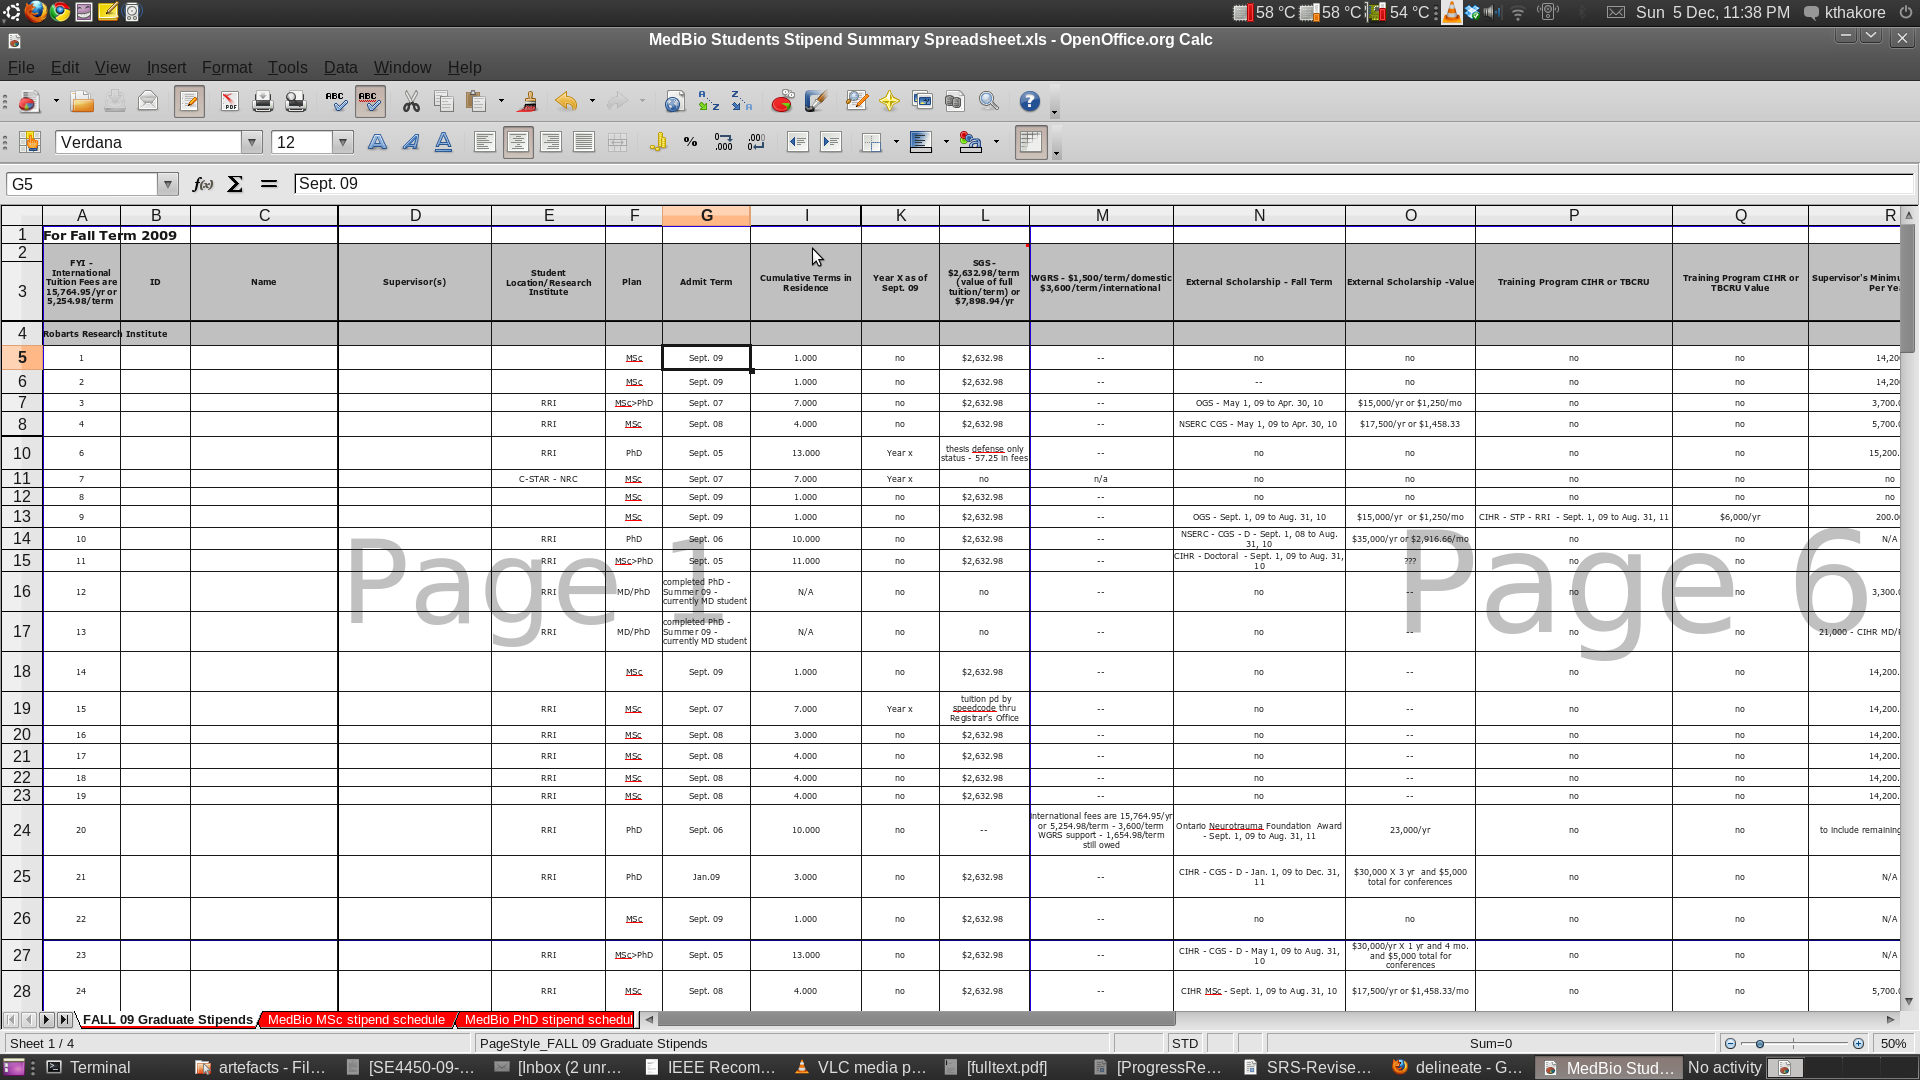
\includegraphics[scale=0.25]{diagrams/Current_System.png}
\caption{Current System}
\label{fig:Curr_Sys}
\end{figure}

\begin{figure}[htp]
\centering
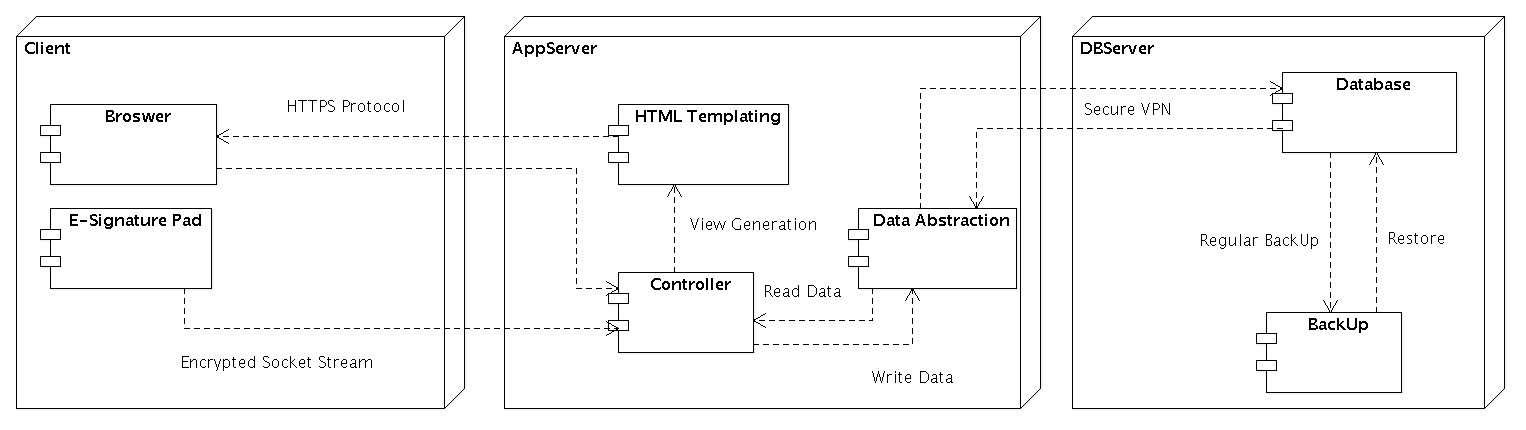
\includegraphics[scale=0.40]{diagrams/SystemOverview.png}
\caption{Proposed System}
\label{fig:New_Sys}
\end{figure}



\section{Overall Description}

\subsection{Product perspective}
The product will be self contained as it is responsible form User Interface, Application and Data Storage.
Figure \ref{fig:New_Sys} again describes the perspective of the system.
The product will have the following constraints:
\begin{itemize}
\item User Interface: The specifications of each view of the user interface will be provided for this project.
\item Hardware Interface: The system will be using a Wacom tablet as a hardware to acquire signatures.
\item Software interfaces: The system will have to employ several software interfaces.
\begin{itemize}
\item Application Server: Apache 2.0 will be used to deploy the system with SSL security.
\item VPN Provider: OpenVPN will be used to deploy our system as a self contained virtual private
network.
\item Database Software: A PostgreSQL RDBMS server will be used to run our Data Storage Component of the Software.
\end{itemize}
\end{itemize}
\subsection{Product function}
\subsection{User characteristics}
Figure \ref{users} describes the relation between the users of the systems:
\begin{itemize}
\item General User
\begin{itemize}
\item Faculty
\item Technical Administrator
\item Graduate Student
\end{itemize}
\end{itemize}

\begin{figure}[htp]
\centering
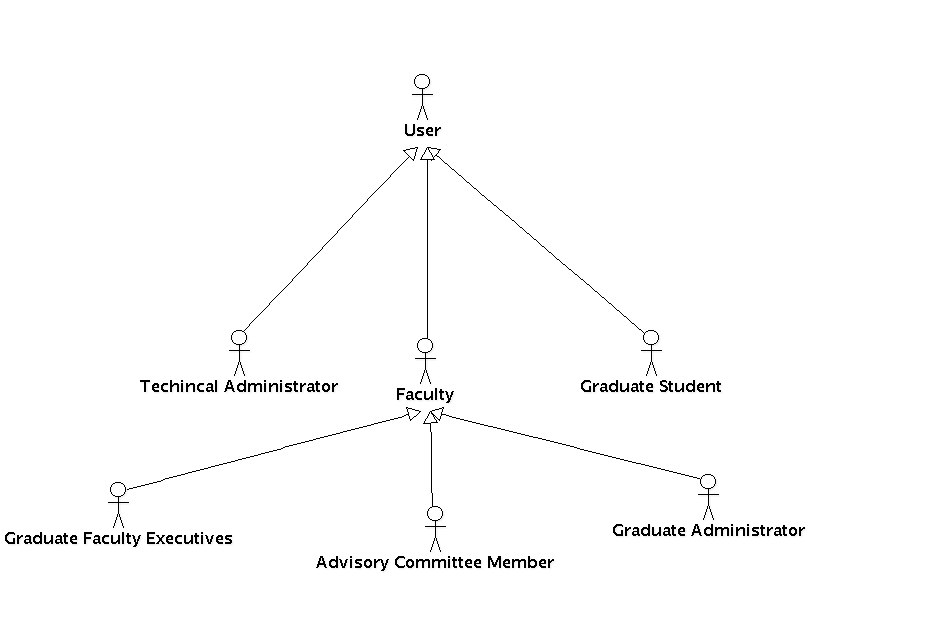
\includegraphics[scale=0.40]{diagrams/use_cases/UserHeirachy_uc.png}
\caption{Users of the System}
\label{users}
\end{figure}

\subsection{Constraints}
\subsection{Assumptions and dependencies}

\section{Specific Requirements}
\subsection{External interface requirements }
\subsection{ Functional requirements }
\subsection{ Performance requirements }
\subsection{ Design constraints }
\subsection{ Software system attributes }
\subsection{ Other requirements }

\clearpage
\newpage 

\listoffigures

\clearpage
\newpage 

\printindex

\end{document}
